\documentclass[12pt,a4paper]{article}

\usepackage{fancyhdr}
\usepackage{graphicx}
\usepackage{placeins}
\usepackage{adjustbox}


\begin{document}

\pagestyle{fancy}
\fancyhf{}
\chead{Short summary report}

\begin{table}[t]
\centering
\caption {rnaQUAST metrics for assembled transcripts. In each row the best values are indicated with \textbf{bold}. For the transcript metrics (rows 4, 5, 6, 9, 13, 25, 26, 27) we highlighted the best \textbf{relative} values i.e. divided by the total number of transcripts in the corresponding assembly.}
\begin{adjustbox}{width=1\textwidth}
\small
\begin{tabular}{|l*{11}{|r}|}
\hline
\textbf{METRICS/TRANSCRIPTS}                            & \textbf{Trinity}       & \textbf{Trans-ABySS}   & \textbf{Oases}         & \textbf{SOAPdenovo-Trans} & \textbf{IDBA-Tran}     & \textbf{Bridger}       & \textbf{BinPacker}     & \textbf{Shannon}       & \textbf{rnaSPAdes}     & \textbf{SPAdes}        \\ \hline\hline
\multicolumn{11}{l}{\bf DATABASE METRICS}                                                 \\ \hline
Genes                                                   & 4497                   & 4497                   & 4497                   & 4497                   & 4497                   & 4497                   & 4497                   & 4497                   & 4497                   & 4497                   \\
Avg. number of exons per isoform                        & 1.015                  & 1.015                  & 1.015                  & 1.015                  & 1.015                  & 1.015                  & 1.015                  & 1.015                  & 1.015                  & 1.015                  \\ \hline
\multicolumn{11}{l}{\bf BASIC TRANSCRIPTS METRICS}                                        \\ \hline
Transcripts                                             & 4403                   & 9555                   & 7364                   & 7007                   & 3803                   & 4254                   & 157                    & 4221                   & 7067                   & 4119                   \\
Transcripts $>$ 500 bp                                  & 1080                   & 1273                   & 1974                   & 1230                   & 1199                   & 1118                   & \textbf{109}           & 1123                   & 1142                   & 1333                   \\
Transcripts $>$ 1000 bp                                 & 347                    & 446                    & 743                    & 439                    & 414                    & 363                    & \textbf{66}            & 372                    & 340                    & 489                    \\ \hline
\multicolumn{11}{l}{\bf ALIGNMENT METRICS}                                                \\ \hline
Aligned                                                 & 4173                   & 9163                   & 7139                   & 6848                   & \textbf{3757}          & 4048                   & 151                    & 4039                   & 6870                   & 3984                   \\
Uniquely aligned                                        & 4074                   & 8992                   & 6921                   & 6799                   & 3732                   & 3883                   & 126                    & 3885                   & 6821                   & 3893                   \\
Multiply aligned                                        & 17                     & 115                    & 26                     & 31                     & 15                     & 16                     & 5                      & 10                     & 21                     & 33                     \\
Unaligned                                               & 230                    & 392                    & 225                    & 159                    & \textbf{46}            & 206                    & 6                      & 182                    & 197                    & 135                    \\ \hline
\multicolumn{11}{l}{\bf ALIGNMENT METRICS FOR NON-MISASSEMBLED TRANSCRIPTS}               \\ \hline
Avg. aligned fraction                                   & 0.99                   & 0.98                   & 0.988                  & 0.994                  & \textbf{0.996}         & 0.991                  & 0.947                  & 0.993                  & 0.992                  & 0.988                  \\
Avg. alignment length                                   & 467.035                & 310.442                & 457.717                & 364.881                & 540.828                & 472.806                & \textbf{1100.774}      & 482.659                & 359.195                & 558.904                \\
Avg. mismatches per transcript                          & 0.368                  & 0.322                  & 0.706                  & \textbf{0.134}         & 0.167                  & 0.265                  & 2.051                  & 0.185                  & 0.212                  & 0.248                  \\ \hline
\multicolumn{11}{l}{\bf ALIGNMENT METRICS FOR MISASSEMBLED (CHIMERIC) TRANSCRIPTS}          \\ \hline
Misassemblies                                           & 13                     & 18                     & 103                    & 1                      & \textbf{0}             & 52                     & 8                      & 54                     & 10                     & 12                     \\ \hline
\multicolumn{11}{l}{\bf ASSEMBLY COMPLETENESS (SENSITIVITY)}                              \\ \hline
Database coverage                                       & \textbf{0.334}         & 0.043                  & \textbf{0.334}         & 0.225                  & 0.183                  & 0.319                  & 0.009                  & 0.318                  & 0.208                  & 0.16                   \\
50\%-assembled genes                                    & \textbf{950}           & 96                     & 916                    & 587                    & 550                    & 920                    & 47                     & 907                    & 469                    & 503                    \\
95\%-assembled genes                                    & 396                    & 32                     & \textbf{414}           & 261                    & 250                    & 382                    & 34                     & 393                    & 187                    & 210                    \\
50\%-covered genes                                      & \textbf{1435}          & 126                    & 1408                   & 824                    & 699                    & 1376                   & 47                     & 1350                   & 707                    & 591                    \\
95\%-covered genes                                      & \textbf{596}           & 38                     & 595                    & 311                    & 294                    & 562                    & 36                     & 565                    & 237                    & 242                    \\
50\%-assembled isoforms                                 & \textbf{950}           & 96                     & 916                    & 587                    & 550                    & 920                    & 47                     & 907                    & 469                    & 503                    \\
95\%-assembled isoforms                                 & 396                    & 32                     & \textbf{414}           & 261                    & 250                    & 382                    & 34                     & 393                    & 187                    & 210                    \\
50\%-covered isoforms                                   & \textbf{1435}          & 126                    & 1408                   & 824                    & 699                    & 1376                   & 47                     & 1350                   & 707                    & 591                    \\
95\%-covered isoforms                                   & \textbf{596}           & 38                     & 595                    & 311                    & 294                    & 562                    & 36                     & 565                    & 237                    & 242                    \\
Mean isoform coverage                                   & 0.647                  & 0.216                  & 0.581                  & 0.447                  & 0.507                  & 0.636                  & \textbf{0.728}         & 0.636                  & 0.42                   & 0.478                  \\
Mean isoform assembly                                   & 0.509                  & 0.191                  & 0.452                  & 0.373                  & 0.45                   & 0.507                  & \textbf{0.719}         & 0.509                  & 0.345                  & 0.436                  \\ \hline
\multicolumn{11}{l}{\bf ASSEMBLY SPECIFICITY}                                             \\ \hline
50\%-matched                                            & \textbf{3358}          & 1001                   & 5029                   & 2941                   & 1543                   & 3212                   & 32                     & 3205                   & 2687                   & 1292                   \\
95\%-matched                                            & \textbf{1619}          & 724                    & 2492                   & 1814                   & 759                    & 1550                   & 2                      & 1535                   & 1756                   & 638                    \\
Unannotated                                             & 303                    & 7494                   & 882                    & 3288                   & 1673                   & 273                    & 53                     & \textbf{255}           & 3511                   & 2075                   \\
Mean fraction of transcript matched                     & 0.746                  & 0.113                  & 0.674                  & 0.411                  & 0.396                  & 0.749                  & 0.272                  & \textbf{0.751}         & 0.38                   & 0.322                  \\ \hline
\end{tabular}
\end{adjustbox}
\end{table}

\FloatBarrier
\clearpage
\lfoot{generated by rnaQUAST}

\begin{figure}[t]
\centering
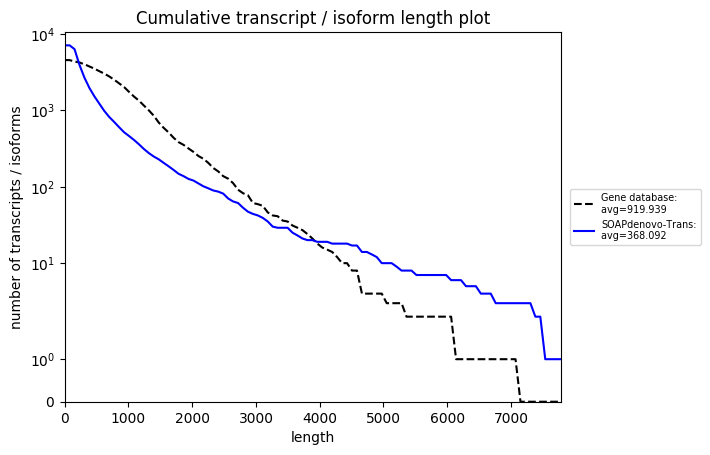
\includegraphics[width = \linewidth]{/mnt/dessertlocal/projects/transcriptome_assembly/review/evaluation/rna-quast/eco/comparison_output/transcript_length.png}
\caption{Plot showing cumulative transcript length distribution. Each point represents the number of transcripts in the assembly with the corresponding length or longer; black dashed line corresponds to the database isoforms; the plot is given in logarithmic scale.}
\end{figure}
\FloatBarrier
\clearpage


\begin{figure}[t]
\centering
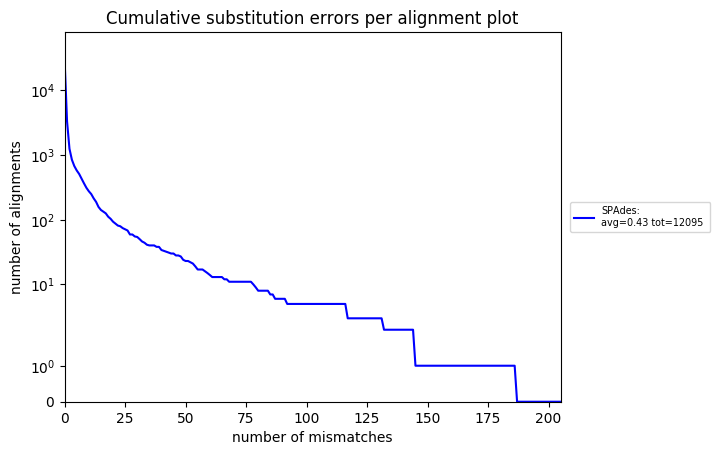
\includegraphics[width = \linewidth]{/mnt/dessertlocal/projects/transcriptome_assembly/review/evaluation/rna-quast/eco/comparison_output/mismatch_rate.png}
\caption{Plot showing cumulative substitution errors per alignment distribution. Each point represents the number of alignments with the corresponding number of mismatches or greater; the plot is given in logarithmic scale.}
\end{figure}
\FloatBarrier
\clearpage


\begin{figure}[t]
\centering
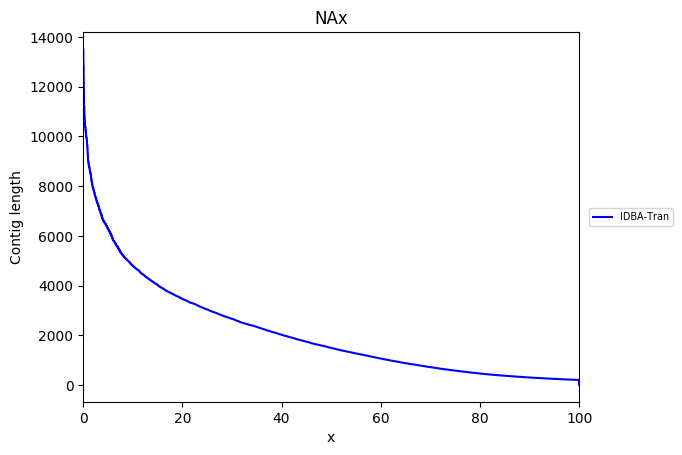
\includegraphics[width = \linewidth]{/mnt/dessertlocal/projects/transcriptome_assembly/review/evaluation/rna-quast/eco/comparison_output/NAx.png}
\caption{Nx plot for transcripts. Nx is a maximal number $N$, such that the total length of all transcripts longer than $N$ bp is at least $x\%$ of the total length of all transcripts.}
\end{figure}
\FloatBarrier
\clearpage


\begin{figure}[t]
\centering
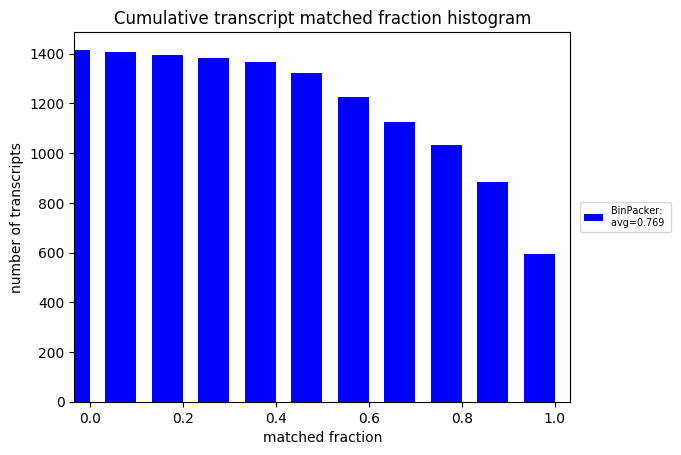
\includegraphics[width = \linewidth]{/mnt/dessertlocal/projects/transcriptome_assembly/review/evaluation/rna-quast/eco/comparison_output/x-matched.png}
\caption{Plot showing cumulative transcript match histogram. Each bar represents the number of transcripts with matched fraction equal to or greater than the value on $x$ axis; transcript matched fraction is calculated as the number of its bases covering an isoform divided by the transcript length.}
\end{figure}
\FloatBarrier
\clearpage


\begin{figure}[t]
\centering
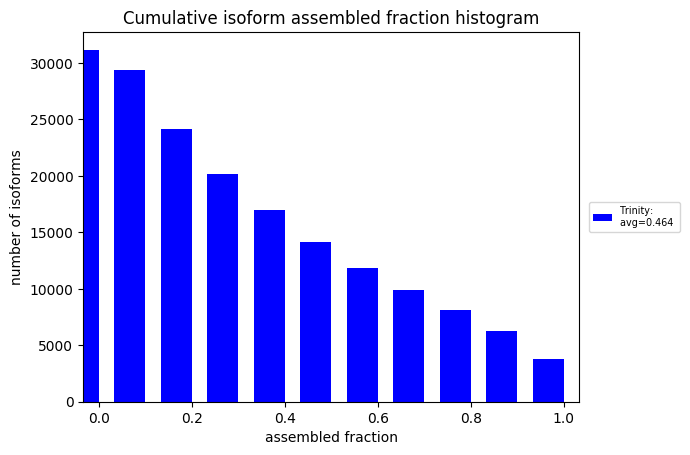
\includegraphics[width = \linewidth]{/mnt/dessertlocal/projects/transcriptome_assembly/review/evaluation/rna-quast/eco/comparison_output/x-assembled.png}
\caption{Plot showing cumulative isoform assembly histogram. Each bar represents the number of isoforms with assembled fraction equal to or greater than the value on $x$ axis; isoform assembled fraction is calculated as the maximum number of captured by single assembled transcript bases divided by the total isoform length.}
\end{figure}
\FloatBarrier
\clearpage


\begin{figure}[t]
\centering
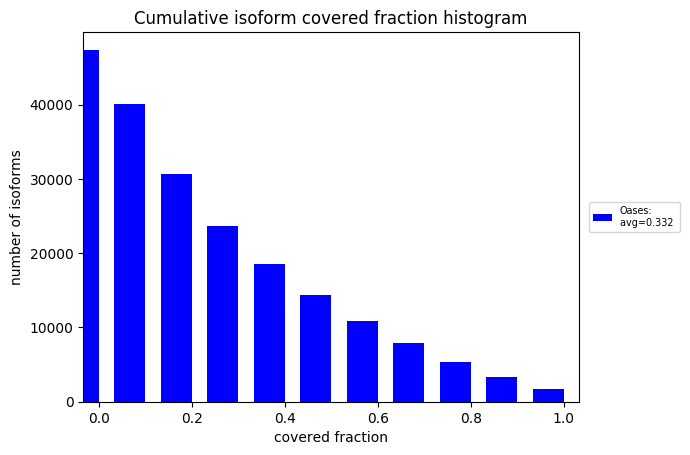
\includegraphics[width = \linewidth]{/mnt/dessertlocal/projects/transcriptome_assembly/review/evaluation/rna-quast/eco/comparison_output/x-covered.png}
\caption{Plot showing cumulative isoform coverage histogram. Each bar represents the number of isoforms with covered fraction equal to or greater than the value on $x$ axis; isoform covered fraction is calculated as the number of covered bases (by all transcripts in the assembly) divided by the total isoform length.}
\end{figure}
\FloatBarrier
\clearpage


\end{document}
